\section{Capítulo 5 -- Estruturas de repetição}

Imagine escrever um programa que mostra a tabuada do 7. Com o que vimos até aqui, seriam dez comandos \texttt{cout} quase iguais. E se fossem as notas de uma turma de 40 alunos? Ou de uma escola com 2 mil? Computadores são extraordinários justamente em repetir uma tarefa milhares ou bilhões de vezes, sem cansar e sem errar. As \textbf{estruturas de repetição} (ou \textbf{laços}, do inglês \textit{loops}) executam um bloco de comandos várias vezes, enquanto uma condição for verdadeira. Neste capítulo você vai conhecer os três laços do C++ e do Portugol, os padrões de uso que aparecem em quase todo programa (contadores, acumuladores, maior e menor valor) e como evitar o erro mais típico das repetições: o laço que nunca termina.

\subsection{5.1 Repetição com teste no início: while}

O \texttt{while} (``enquanto'') testa uma condição; se ela for verdadeira, executa o bloco e volta a testar. Quando a condição fica falsa, o laço termina e o programa segue. Cada execução do bloco é chamada de \textbf{iteração} (ou volta).

\begin{center}
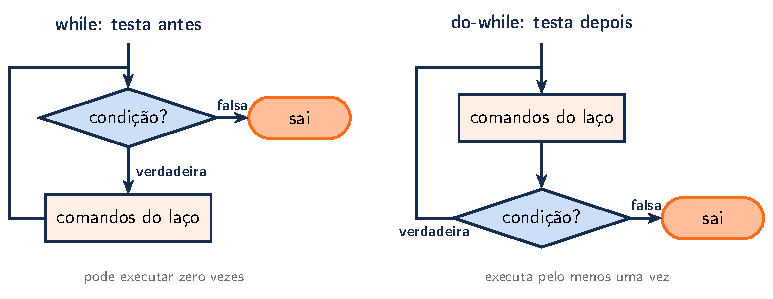
\includegraphics[width=0.85\linewidth,keepaspectratio]{imagens/capitulo-05_while.pdf}
\end{center}

Como o teste vem antes, se a condição já começar falsa o bloco não é executado nenhuma vez. E algo dentro do bloco precisa, em algum momento, tornar a condição falsa; senão o laço nunca termina.

\begin{codigo}
\begin{Verbatim}[breaklines=true, breaksymbolleft={}, fontsize=\footnotesize]
#include <iostream>
using namespace std;

int main() {
    int contador = 5;
    while (contador > 0) {
        cout << contador << " ";
        contador--;               // aproxima o laço do fim
    }
    cout << "Fogo!" << endl;      // 5 4 3 2 1 Fogo!
    return 0;
}
\end{Verbatim}
\end{codigo}

Em Portugol, o mesmo laço é escrito com \texttt{enquanto ... faca ... fimenquanto}:

\begin{codigo}
\begin{Verbatim}[breaklines=true, breaksymbolleft={}, fontsize=\footnotesize]
algoritmo "ContagemRegressiva"
var
   contador: inteiro
inicio
   contador <- 5
   enquanto contador > 0 faca
      escreva(contador, " ")
      contador <- contador - 1
   fimenquanto
   escreval("Fogo!")
fimalgoritmo
\end{Verbatim}
\end{codigo}

\subsubsection{Laço controlado por sentinela}

O \texttt{while} é o laço certo quando \textbf{não se sabe de antemão} quantas vezes repetir. Um caso muito comum é ler dados até que o usuário digite um valor especial, chamado de \textbf{sentinela}, que indica o fim. O valor da sentinela não pode ser um dado válido: para somar valores positivos, o 0 funciona bem.

\begin{codigo}
\begin{Verbatim}[breaklines=true, breaksymbolleft={}, fontsize=\footnotesize]
algoritmo "SomarCompras"
var
   valor, soma, quantos: inteiro
inicio
   soma <- 0
   quantos <- 0
   escreva("Valores das compras (0 para terminar): ")
   leia(valor)                  // primeira leitura, antes do laço
   enquanto valor <> 0 faca
      soma <- soma + valor
      quantos <- quantos + 1
      leia(valor)               // próxima, no fim do bloco
   fimenquanto
   escreval(quantos, " compras, total ", soma)
fimalgoritmo
\end{Verbatim}
\end{codigo}

Repare no padrão: uma leitura antes do laço e outra no fim do bloco. Assim, a condição sempre testa o valor recém-lido, e a sentinela nunca entra na soma.

Em C++, o mesmo padrão costuma ser escrito de forma mais curta, com a leitura dentro da própria condição. A expressão \texttt{cin >> valor} lê o valor e, além disso, resulta em verdadeiro se a leitura deu certo e em falso se falhou, por exemplo quando a entrada acabou ou o usuário digitou uma letra. Assim, o laço para tanto na sentinela quanto em uma entrada que termina sem ela, o que evita um laço infinito:

\begin{codigo}
\begin{Verbatim}[breaklines=true, breaksymbolleft={}, fontsize=\footnotesize]
#include <iostream>
using namespace std;

int main() {
    int valor, soma = 0, quantos = 0;
    cout << "Valores das compras (0 para terminar): ";
    while (cin >> valor && valor != 0) {   // lê e testa
        soma += valor;
        quantos++;
    }
    cout << quantos << " compras, total " << soma << endl;
    return 0;
}
// Entrada: 30 45 25 0  ->  3 compras, total 100
\end{Verbatim}
\end{codigo}

\subsection{5.2 Repetição com teste no fim: do-while}

O \texttt{do-while} (``faça enquanto'') executa o bloco \textbf{primeiro} e só depois testa a condição. Por isso, o bloco é executado \textbf{pelo menos uma vez}. Ele é ideal quando a primeira execução é obrigatória, como pedir um dado e repetir o pedido enquanto ele for inválido.

\begin{codigo}
\begin{Verbatim}[breaklines=true, breaksymbolleft={}, fontsize=\footnotesize]
#include <iostream>
using namespace std;

int main() {
    double nota;
    do {
        cout << "Nota (0 a 10): ";
        cin >> nota;
        if (nota < 0 || nota > 10) {
            cout << "Nota inválida, tente de novo." << endl;
        }
    } while (nota < 0 || nota > 10);   // repete se inválida
    cout << "Nota registrada: " << nota << endl;
    return 0;
}
// Entrada: 30, depois 7.5  ->  Nota inválida...
//                              Nota registrada: 7.5
\end{Verbatim}
\end{codigo}

Atenção ao ponto e vírgula depois do \texttt{while (...)} do \texttt{do-while}: ele é obrigatório, ao contrário do \texttt{while} comum.

No Portugol, a estrutura equivalente é \texttt{repita ... ate}, com uma diferença importante: a condição do \texttt{ate} diz quando \textbf{parar}, e não quando continuar. O laço repete \textbf{até} a condição ficar verdadeira. Por isso, ela é o contrário da condição do \texttt{do-while}:

\begin{codigo}
\begin{Verbatim}[breaklines=true, breaksymbolleft={}, fontsize=\footnotesize]
algoritmo "LerNota"
var
   nota: real
inicio
   repita
      escreva("Nota (0 a 10): ")
      leia(nota)
   ate (nota >= 0) e (nota <= 10)    // para quando for válida
   escreval("Nota registrada: ", nota)
fimalgoritmo
\end{Verbatim}
\end{codigo}

\subsection{5.3 Repetição com contador: for}

Quando se sabe \textbf{quantas vezes} repetir, o \texttt{for} (``para'') é o laço mais claro, porque reúne em uma única linha as três partes de um laço com contador: a inicialização, a condição e a atualização.

\begin{center}
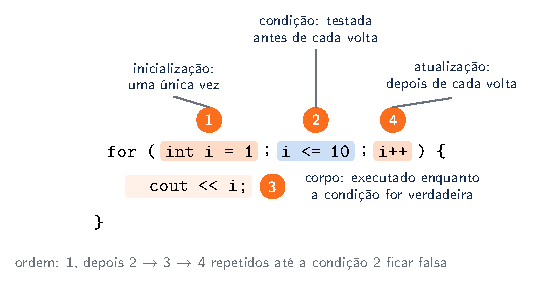
\includegraphics[width=0.75\linewidth,keepaspectratio]{imagens/capitulo-05_for.pdf}
\end{center}

\begin{codigo}
\begin{Verbatim}[breaklines=true, breaksymbolleft={}, fontsize=\footnotesize]
#include <iostream>
using namespace std;

int main() {
    int n;
    cout << "Tabuada do: ";
    cin >> n;
    for (int i = 1; i <= 10; i++) {
        cout << n << " x " << i << " = " << n * i << endl;
    }

    for (int i = 10; i >= 0; i -= 2) {   // de 10 até 0, de 2 em 2
        cout << i << " ";
    }
    cout << endl;                        // 10 8 6 4 2 0
    return 0;
}
\end{Verbatim}
\end{codigo}

A variável \texttt{i}, declarada dentro do \texttt{for}, só existe dentro do laço. O contador pode começar e terminar em qualquer valor, crescer ou diminuir, e andar de um em um ou em passos maiores: tudo depende das três partes.

No Portugol, o laço com contador é o \texttt{para ... de ... ate ... faca}, com um \texttt{passo} opcional (que vale 1 quando omitido):

\begin{codigo}
\begin{Verbatim}[breaklines=true, breaksymbolleft={}, fontsize=\footnotesize]
algoritmo "Tabuada"
var
   n, i: inteiro
inicio
   escreva("Tabuada do: ")
   leia(n)
   para i de 1 ate 10 faca
      escreval(n, " x ", i, " = ", n * i)
   fimpara
   para i de 10 ate 0 passo -2 faca
      escreva(i, " ")
   fimpara
fimalgoritmo
\end{Verbatim}
\end{codigo}

Os três laços são equivalentes, no sentido de que qualquer repetição pode ser escrita com qualquer um deles. A escolha é sobre clareza:

\begin{center}
\begin{tabular}{@{}p{0.22\linewidth}p{0.3\linewidth}p{0.38\linewidth}@{}}
\toprule
\rowcolor{headergray}
\tblheader{Laço} & \tblheader{Portugol} & \tblheader{Use quando} \\
\midrule
\texttt{for} & \texttt{para ... fimpara} & o número de repetições é conhecido \\
\rowcolor{rowgray} \texttt{while} & \texttt{enquanto ... fimenquanto} & depende de algo que só se sabe durante a execução \\
\texttt{do-while} & \texttt{repita ... ate} & a primeira execução é obrigatória \\
\bottomrule
\end{tabular}
\end{center}

\subsection{5.4 Contadores, acumuladores, maior e menor}

Quase todo laço que processa dados usa um ou mais destes quatro padrões:

\begin{itemize}
  \item \textbf{Contador}: uma variável que começa em 0 e soma 1 a cada vez que algo acontece (\texttt{quantos++}). Com uma condição, conta só alguns casos: quantos aprovados, quantos negativos.
  \item \textbf{Acumulador}: uma variável que começa em 0 e soma um valor a cada volta (\texttt{soma += nota}). No fim, guarda o total. Para multiplicar, o acumulador começa em 1.
  \item \textbf{Maior valor}: compara cada dado com o maior visto até agora e o substitui quando encontra um maior.
  \item \textbf{Menor valor}: o mesmo, com a comparação invertida.
\end{itemize}

O programa abaixo usa os quatro para analisar as notas de uma turma:

\begin{codigo}
\begin{Verbatim}[breaklines=true, breaksymbolleft={}, fontsize=\footnotesize]
#include <iostream>
using namespace std;

int main() {
    int alunos;
    cout << "Quantos alunos? ";
    cin >> alunos;
    double soma = 0;               // acumulador
    int aprovados = 0;             // contador
    double maior = 0, menor = 10;  // os extremos da faixa
    for (int i = 1; i <= alunos; i++) {
        double nota = 0;
        cout << "Nota do aluno " << i << ": ";
        cin >> nota;
        soma += nota;
        if (nota >= 6) aprovados++;
        if (nota > maior) maior = nota;
        if (nota < menor) menor = nota;
    }
    if (alunos > 0) {
        cout << "Média: " << soma / alunos << endl;
        cout << "Aprovados: " << aprovados << endl;
        cout << "Maior: " << maior << ", menor: " << menor
             << endl;
    }
    return 0;
}
// 4 alunos com 7, 4.5, 9 e 6 -> Média: 6.625
// Aprovados: 3    Maior: 9, menor: 4.5
\end{Verbatim}
\end{codigo}

O maior começa em 0 e o menor em 10, os extremos da faixa de notas: assim, a primeira nota lida sempre substitui os dois. Quando não há uma faixa conhecida, a forma mais segura é usar o \textbf{primeiro valor lido} como maior e menor iniciais. O \texttt{if (alunos > 0)} evita dividir por zero quando a turma está vazia.

Um teste de mesa mostra o laço trabalhando, volta a volta, com as notas 7, 4.5, 9 e 6:

\begin{center}
\begin{tabular}{@{}p{0.08\linewidth}p{0.1\linewidth}p{0.12\linewidth}p{0.19\linewidth}p{0.12\linewidth}p{0.12\linewidth}@{}}
\toprule
\rowcolor{headergray}
\tblheader{i} & \tblheader{nota} & \tblheader{soma} & \tblheader{aprovados} & \tblheader{maior} & \tblheader{menor} \\
\midrule
-- & -- & 0 & 0 & 0 & 10 \\
\rowcolor{rowgray} 1 & 7 & 7 & 1 & 7 & 7 \\
2 & 4.5 & 11.5 & 1 & 7 & 4.5 \\
\rowcolor{rowgray} 3 & 9 & 20.5 & 2 & 9 & 4.5 \\
4 & 6 & 26.5 & 3 & 9 & 4.5 \\
\bottomrule
\end{tabular}
\end{center}

\subsection{5.5 Interrompendo um laço: break e continue}

Dois comandos alteram o andamento normal de um laço:

\begin{itemize}
  \item \texttt{break} encerra o laço imediatamente, mesmo que a condição ainda seja verdadeira. É útil quando a resposta já foi encontrada e não faz sentido continuar procurando.
  \item \texttt{continue} pula o resto da iteração atual e passa direto para a próxima.
\end{itemize}

\begin{codigo}
\begin{Verbatim}[breaklines=true, breaksymbolleft={}, fontsize=\footnotesize]
#include <iostream>
using namespace std;

int main() {
    // break: o primeiro múltiplo de 7 maior que 50
    for (int n = 51; n <= 100; n++) {
        if (n % 7 == 0) {
            cout << "Encontrado: " << n << endl;   // 56
            break;                // não precisa olhar o resto
        }
    }

    // continue: soma só os ímpares de 1 a 10
    int soma = 0;
    for (int i = 1; i <= 10; i++) {
        if (i % 2 == 0) {
            continue;                  // pula os pares
        }
        soma += i;
    }
    cout << "Soma dos ímpares: " << soma << endl;   // 25
    return 0;
}
\end{Verbatim}
\end{codigo}

O Portugol do VisuAlg tem o comando \texttt{interrompa}, equivalente ao \texttt{break}, mas não tem equivalente ao \texttt{continue}. Use os dois com moderação: um laço com muitas saídas no meio é difícil de acompanhar. Muitas vezes, uma condição melhor no próprio laço ou um \texttt{if} resolvem o problema de forma mais clara.

\subsection{5.6 Laços aninhados}

Um laço pode estar dentro de outro. Para cada volta do laço de fora, o laço de dentro é executado \textbf{inteiro}. Se o de fora dá 4 voltas e o de dentro, 5, o bloco mais interno é executado $4 \times 5 = 20$ vezes. Laços aninhados aparecem sempre que os dados têm linhas e colunas: tabelas, matrizes (Capítulo 7), imagens.

\begin{codigo}
\begin{Verbatim}[breaklines=true, breaksymbolleft={}, fontsize=\footnotesize]
#include <iostream>
#include <iomanip>     // setw
using namespace std;

int main() {
    // um triângulo: a linha i tem i asteriscos
    for (int linha = 1; linha <= 4; linha++) {
        for (int j = 1; j <= linha; j++) {
            cout << "*";
        }
        cout << endl;
    }

    // a tabela de multiplicação de 1 a 5
    for (int i = 1; i <= 5; i++) {
        for (int j = 1; j <= 5; j++) {
            cout << setw(4) << i * j;  // 4 posições por número
        }
        cout << endl;
    }
    return 0;
}
\end{Verbatim}
\end{codigo}

A saída mostra o triângulo e a tabela, com as colunas alinhadas pelo \texttt{setw(4)}, que reserva 4 posições para cada número:

\begin{codigo}
\begin{Verbatim}[breaklines=true, breaksymbolleft={}, fontsize=\footnotesize]
// saída
*
**
***
****
   1   2   3   4   5
   2   4   6   8  10
   3   6   9  12  15
   4   8  12  16  20
   5  10  15  20  25
\end{Verbatim}
\end{codigo}

Repare que o limite do laço de dentro, no triângulo, depende da variável do laço de fora (\texttt{j <= linha}): é isso que faz cada linha ter um asterisco a mais.

\subsection{5.7 O laço que não termina}

Um \textbf{laço infinito} acontece quando a condição nunca fica falsa. O programa trava, ou fica mostrando a mesma coisa sem parar, e precisa ser interrompido à força (no terminal, com Ctrl+C). As causas mais comuns são:

\begin{itemize}
  \item esquecer de atualizar a variável da condição, como o \texttt{contador--} do \texttt{while};
  \item atualizar na direção errada: \texttt{for (int i = 10; i >= 0; i++)} se afasta da condição de parada em vez de se aproximar;
  \item usar uma condição que nunca pode ser satisfeita, como \texttt{while (x != 10)} com \texttt{x} andando de 3 em 3 a partir de 0: ele passa por 9 e 12, mas nunca vale 10.
\end{itemize}

O erro oposto também é comum: o laço que executa \textbf{uma vez a mais ou a menos} do que deveria, por usar \texttt{<} no lugar de \texttt{<=}, ou começar em 0 no lugar de 1. Ele é tão frequente que tem nome em inglês, \textit{off-by-one}. Antes de confiar em um laço, verifique a primeira e a última volta: com que valor do contador elas acontecem?

\subsection{5.8 Um programa completo: números primos}

Um número é \textbf{primo} quando é maior que 1 e só é divisível por 1 e por ele mesmo: 2, 3, 5, 7, 11, 13\ldots{} Para saber se \texttt{n} é primo, basta procurar um divisor entre 2 e \texttt{n - 1}; se algum dividir, ele não é primo.

Dá para procurar bem menos. Se \texttt{n} tiver um divisor maior que sua raiz quadrada, terá também um menor que ela: $36 = 4 \times 9$, e o 4 é menor que $\sqrt{36} = 6$. Então basta testar os divisores \texttt{d} enquanto \texttt{d * d <= n}. Para um número perto de um milhão, isso reduz a busca de cerca de um milhão de divisões para mil. E, assim que um divisor aparece, o \texttt{break} encerra a busca.

\begin{codigo}
\begin{Verbatim}[breaklines=true, breaksymbolleft={}, fontsize=\footnotesize]
algoritmo "Primo"
var
   n, d: inteiro
   primo: logico
inicio
   escreva("Número: ")
   leia(n)
   primo <- n >= 2
   d <- 2
   enquanto (d * d <= n) e primo faca
      se n mod d = 0 entao
         primo <- falso
      fimse
      d <- d + 1
   fimenquanto
   se primo entao
      escreval(n, " é primo")
   senao
      escreval(n, " não é primo")
   fimse
fimalgoritmo
\end{Verbatim}
\end{codigo}

\begin{codigo}
\begin{Verbatim}[breaklines=true, breaksymbolleft={}, fontsize=\footnotesize]
#include <iostream>
using namespace std;

int main() {
    int n;
    cout << "Número: ";
    cin >> n;
    bool primo = n >= 2;              // 0 e 1 não são primos
    for (int d = 2; d * d <= n; d++) {
        if (n % d == 0) {
            primo = false;            // achou um divisor
            break;
        }
    }
    cout << n << (primo ? " é primo" : " não é primo") << endl;
    return 0;
}
// 2 -> é primo     9 -> não é primo    97 -> é primo
// 1 -> não é primo     1000003 -> é primo
\end{Verbatim}
\end{codigo}

O Portugol usa a própria variável \texttt{primo} na condição do \texttt{enquanto} para parar a busca, em vez de um comando de interrupção: as duas formas são corretas. Para testar, inclua os casos especiais: 0, 1 e 2 (o único primo par), um quadrado perfeito como 9 ou 49 (que só tem o divisor exatamente na raiz e testa o \texttt{<=}) e um primo grande.

\subsection{Erros Comuns}

\begin{itemize}
  \item \textbf{Esquecer de atualizar a variável da condição.} O laço nunca termina.
  \item \textbf{Errar o limite por um.} \texttt{i < 10} dá 10 voltas começando em 0, mas 9 começando em 1. Confira a primeira e a última volta.
  \item \textbf{Colocar ponto e vírgula depois do \texttt{for} ou do \texttt{while}.} \texttt{for (...);} repete um comando vazio, e o bloco abaixo executa uma única vez.
  \item \textbf{Esquecer o ponto e vírgula do \texttt{do-while}.} Ele é obrigatório depois de \texttt{while (condição)}.
  \item \textbf{Inverter a condição do \texttt{repita ... ate}.} No Portugol ela diz quando parar, ao contrário do \texttt{do-while}.
  \item \textbf{Não inicializar contadores e acumuladores.} Uma soma que começa com lixo dá lixo. Comece em 0 (ou em 1, para produtos).
  \item \textbf{Inicializar o maior ou o menor com um valor possível.} Começar o maior em 0 falha se todos os dados forem negativos. Use um valor fora da faixa ou o primeiro dado lido.
  \item \textbf{Somar a sentinela.} No laço com sentinela, leia antes do laço e no fim do bloco (ou, em C++, dentro da condição), para que o valor de parada nunca seja processado.
  \item \textbf{Dividir pela quantidade sem verificar se ela é zero.} Uma média de nenhum valor não existe.
\end{itemize}
